\documentclass[fleqn, a4paper, 12pt, twoside]{article}
\usepackage{exsheets}
\usepackage{amsmath, amssymb, amsthm} %standard AMS packages
\usepackage{marginnote} %marginnotes
\usepackage{gensymb} %miscellaneous symbols
\usepackage{commath} %differential symbols
\usepackage{xcolor} %colours
\usepackage{cancel} %cancelling terms
\usepackage[free-standing-units]{siunitx} %formatting units
\usepackage{tikz, pgfplots} %diagrams
	\usetikzlibrary{calc, hobby, patterns, intersections}
\usepackage{graphicx} %inserting graphics
\usepackage{hyperref} %hyperlinks
\usepackage{datetime} %date and time
\usepackage{ulem} %underline for \emph{}
\usepackage{xfrac, lmodern} %inline fractions
\usepackage{enumerate, enumitem} %numbered lists
\usepackage{float} %inserting floats
\usepackage{tabularx}

\newcommand\numberthis{\addtocounter{equation}{1}\tag{\theequation}} %adds numbers to specific equations in non-numbered list of equations

\newcommand{\AxisRotator}[1][rotate=0]{
	\tikz [x=0.25cm,y=0.60cm,line width=.2ex,-stealth,#1] \draw (0,0) arc (-150:150:1 and 1);%
} %rotation symbols on axes

\theoremstyle{definition}
\newtheorem{example}{Example}
\newtheorem{definition}{Definition}

\theoremstyle{theorem}
\newtheorem{theorem}{Theorem}

\newcommand{\curl}{\mathrm{curl\,}}

\makeatletter
\@addtoreset{section}{part} %resets section numbers in new part
\makeatother

\makeatletter
\newcommand*{\relrelbarsep}{.386ex}
\newcommand*{\relrelbar}{%
  \mathrel{%
    \mathpalette\@relrelbar\relrelbarsep
  }%
}
\newcommand*{\@relrelbar}[2]{%
  \raise#2\hbox to 0pt{$\m@th#1\relbar$\hss}%
  \lower#2\hbox{$\m@th#1\relbar$}%
}
\providecommand*{\rightrightarrowsfill@}{%
  \arrowfill@\relrelbar\relrelbar\rightrightarrows
}
\providecommand*{\leftleftarrowsfill@}{%
  \arrowfill@\leftleftarrows\relrelbar\relrelbar
}
\providecommand*{\xrightrightarrows}[2][]{%
  \ext@arrow 0359\rightrightarrowsfill@{#1}{#2}%
}
\providecommand*{\xleftleftarrows}[2][]{%
  \ext@arrow 3095\leftleftarrowsfill@{#1}{#2}%
}
\makeatother

\newcommand\blfootnote[1]{%
	\begingroup
	\renewcommand\thefootnote{}\footnote{#1}%
	\addtocounter{footnote}{-1}%
	\endgroup
}

\SetupExSheets{solution/print = true} %prints all solutions by default
%opening
\title{Differential and Integral Calculus}
\author{Aakash Jog}
\date{2014-15}

\begin{document}

\maketitle
%\setlength{\mathindent}{0pt}

\blfootnote
{	
	\begin{figure}[H]
		
\includegraphics[height = 12pt]{cc.eps}
		\includegraphics[height = 12pt]{by.eps}
		\includegraphics[height = 12pt]{nc.eps}
		\includegraphics[height = 12pt]{sa.eps}
	\end{figure}
	This work is licensed under the Creative Commons Attribution-NonCommercial-ShareAlike 4.0 International License. To view a copy of this license, visit \url{http://creativecommons.org/licenses/by-nc-sa/4.0/}.
} %CC-BY-NC-SA licencse

\tableofcontents

\newpage
\section{Lecturer Information}

\textbf{Dr. Yakov Yakubov}\\
~\\
Office: Schreiber 233\\
Telephone: {\href{tel:+97236405357}{+972 3-640-5357}\\
E-mail: \href{mailto:yakubov@post.tau.ac.il}{yakubov@post.tau.ac.il}\\

\section{Required Reading}

Protter and Morrey: \textit{A first Course in Real Analysis}, UTM Series, Springer-Verlag, 1991

\section{Additional Reading}

Thomas and Finney, \textit{Calculus and Analytic Geometry}, 9th edition, Addison-Wesley, 1996

\newpage
\part{Sequences and Series}

\section{Sequences}

\begin{definition}[Sequence]
	A sequence of real numbers is a set of numbers which are written in some order. There are infinitely many terms in a sequence. It is denoted by $\{a_n\}_{n = 1}^{\infty}$ or $\{a_n\}$.
\end{definition}

\begin{example}
	$1, \dfrac{1}{2}, \dfrac{1}{3}, \dots$ is called the harmonic sequence.
	\begin{equation*}
		a_n = \dfrac{1}{n}
	\end{equation*}
\end{example}

\begin{example}
	$1, -\dfrac{1}{2}, \dfrac{1}{3}, \dots$ is called the alternating harmonic sequence.
	\begin{equation*}
		a_n = (-1)^{n + 1} \dfrac{1}{n}
	\end{equation*}
\end{example}

\begin{example}
	$\dfrac{1}{2}, \dfrac{2}{3}, \dfrac{3}{4}, \dots$
	\begin{equation*}
		a_n = \dfrac{n}{n + 1}
	\end{equation*}
\end{example}

\begin{example}
	$\dfrac{2}{3}, \dfrac{3}{9}, \dfrac{4}{27}, \dots$
	\begin{align*}
		a_n = \dfrac{n + 1}{3^n}
	\end{align*}
\end{example}

\begin{example}
	The Fibonacci sequence is given by
	\begin{equation*}
		f_n =
			\begin{cases}
				1 &;\quad n = 1, 2\\
				f_{n - 1} + f_{n - 2} &;\quad n \geq 3\\
			\end{cases}
	\end{equation*}
\end{example}

\begin{example}
	A geometric sequence is given by
	\begin{equation*}
		a_n = a_1 q^{n - 1}
	\end{equation*}
	where $q$ is called the common ratio.
\end{example}

\begin{example}
	A geometric sequence is given by
	\begin{equation*}
		a_n = a_1 + d(n - 1)
	\end{equation*}
	where $d$ is called the common difference.
\end{example}

\begin{definition}[Equal sequences]
	Two sequences $\{a_n\}$ and $\{b_n\}$ are said to be equal if $a_n = b_n$, $\forall n \in \mathbb{N}$.
\end{definition}

\begin{definition}[Sequences bounded from above]
	$\{a_n\}$ is said to be bounded from above if $\exists M \in \mathbb{R}$, s.t. $a_n \leq M$, $\forall n \in \mathbb{N}$.
	Each such $M$ is called an upper bound of $\{a_n\}$.
\end{definition}

\begin{definition}[Sequences bounded from below]
	$\{a_n\}$ is said to be bounded from below if $\exists m \in \mathbb{R}$, s.t. $a_n \geq M$, $\forall n \in \mathbb{N}$.
	Each such $M$ is called an lower bound of $\{a_n\}$.
\end{definition}

\begin{definition}
	$\{a_n\}$ is said to be bounded if it is bounded from below and bounded from above.
\end{definition}

\begin{example}
	The sequence $a_n = n^2 + 2$ is not bounded from above but is bounded from below, by all $m \leq 3$.
\end{example}

\begin{example}
	$\left\{ \dfrac{2n - 1}{3n} \right\}$ is bounded.
	\begin{equation*}
		m = 0 \leq \dfrac{2n - 1}{3n} \leq \dfrac{2n}{3n} = \dfrac{2}{3} = M
	\end{equation*}
\end{example}

\begin{definition}[Monotonic increasing sequence]
	A sequence $\{a_n\}$ is called monotonic increasing if $\exists n_0 \in \mathbb{N}$, s.t. $a_n \leq a_{n + 1}$, $\forall n \geq n_0$.
\end{definition}

\begin{definition}[Monotonic decreasing sequence]
	A sequence $\{a_n\}$ is called monotonic decreasing if $\exists n_0 \in \mathbb{N}$, s.t. $a_n \geq a_{n + 1}$, $\forall n \geq n_0$.
\end{definition}

\begin{definition}[Strongly increasing sequence]
	A sequence $\{a_n\}$ is called monotonic increasing if $\exists n_0 \in \mathbb{N}$, s.t. $a_n < a_{n + 1}$, $\forall n \geq n_0$.
\end{definition}

\begin{definition}[Strongly decreasing sequence]
	A sequence $\{a_n\}$ is called monotonic decreasing if $\exists n_0 \in \mathbb{N}$, s.t. $a_n > a_{n + 1}$, $\forall n \geq n_0$.
\end{definition}

\begin{example}
	The sequence $\left\{ \dfrac{n^2}{2^n} \right\}$ is strongly decreasing.
	However, this is not evident by observing the first few terms.
	$\dfrac{1}{2}, 1, \dfrac{9}{8}, 1, \dfrac{25}{32}, \dots$
	\begin{align*}
		a_n &> a_{n + 1}\\
		\iff \dfrac{n^2}{2^n} &> \dfrac{(n + 1)^2}{2^{n + 1}}\\
		\iff 2 n^2 &> (n + 1)^2\\
		\iff \sqrt{2} n &> n + 1\\
		\iff n(\sqrt{2} - 1) &> 1\\
		\iff n &> \dfrac{1}{\sqrt{2} - 1}\\
		\iff n &> 3
	\end{align*}
\end{example}

\begin{question}
	Is $a_n = (-1)^n$ monotonic?
\end{question}

\begin{solution}[print]
	The sequence $-1, 1, -1, 1, \dots$ is not monotonic.
\end{solution}

\subsection{Limit of a Sequence}

\begin{definition}
	Let $\{a_n\}$ be a given sequence.
	A number $L$ is said to be the limit of the sequence if $\forall \varepsilon > 0$, $\exists n_0 \in \mathbb{N}$, s.t. $|a_n - L| < \varepsilon$, $\forall n \geq n_0$.
	That is, there are infinitely many terms inside the interval and a finite number of terms outside it.
\end{definition}

\begin{example}
	The sequence $\{\dfrac{1}{n}\}$ tends to 0, i.e. for any open interval $(-\varepsilon, \varepsilon)$, there are finite number of terms of the sequence outside the interval, and therefore there are infinitely many terms inside the interval.
\end{example}

\begin{question}
	Prove
	\begin{equation*}
		\lim\limits_{n \to \infty} \dfrac{n + 2}{2n - 1} = \dfrac{1}{2}
	\end{equation*}
\end{question}

\begin{solution}
	$\forall \varepsilon > 0$, $\exists n_0 \in \mathbb{N}$
\end{solution}

\begin{question}
	Prove that 2 is not a limit of $\left\{ \dfrac{3n + 1}{n} \right\}$.
\end{question}

\begin{solution}
	If possible, let 
	\begin{align*}
		\lim\limits_{n \to \infty} \dfrac{3n + 1}{n} = 2
	\end{align*}
	Then, $\forall \varepsilon > 0$, $\exists n_0 \in \mathbb{N}$, s.t. $\left| \dfrac{3n + 1}{n} - 2 \right| < \varepsilon$, $\forall n \geq n_0$.
	However,
	\begin{equation*}
		\left| \dfrac{3n + 1}{n} - 2 \right| = 1 + \dfrac{1}{n} > 1
	\end{equation*}
	This is a contradiction for $\varepsilon = \dfrac{1}{2}$.
	Therefore, 2 is not a limit.
\end{solution}

\begin{theorem}
	If a sequence $\{a_n\}$ has a limit $L$ then the limit is unique.
	\label{uniquness of a limit}
\end{theorem}

\begin{proof}
	If possible let there exist two limits $L_1$ and $L_2$.
	Therefore, $\forall \varepsilon > 0$, there exist a finite number of terms in the interval $(L_1 - \varepsilon, L_1 + \varepsilon)$.
	Therefore, there exist a finite number of terms in the interval $(L_2 - \varepsilon, L_2 + \varepsilon)$.
	This contradicts the definition of a limit.
	Therefore, the limit is unique.
\end{proof}

\begin{theorem}
	If a sequence $\{a_n\}$ has limit $L$, then the sequence is bounded.
	\label{existence of limit implies boundedness}
\end{theorem}

\begin{theorem}
	Let
	\begin{align*}
		\lim\limits_{n \to \infty} a_n &= a\\
		\lim\limits_{n \to \infty} b_n &= b
	\end{align*}
	and let $c$ be a constant.
	Then,
	\begin{align*}
		\lim c &= c\\
		\lim (c a_n) &= c \lim a_n\\
		\lim (a_n \pm b_n) &= \lim a_n \pm \lim b_n\\
		\lim (a_n b_n) &= \lim a_n \lim b_n\\
		\lim (\dfrac{a_n}{b_n}) &= \dfrac{\lim a_n}{\lim b_n} \quad (\textnormal{ if } \lim b \neq 0)
	\end{align*}
	\label{limit arithmetic}
\end{theorem}

\begin{theorem}
	Let $\{b_n\}$ be bounded and let $\lim a_n = 0$. Then,
	\begin{equation*}
		\lim (a_n b_n) = 0
	\end{equation*}
\end{theorem}

\begin{theorem}[Sandwich Theorem]
	Let $\{a_n\}$, $\{b_n\}$, $\{c_n\}$ be three sequences. If
	\begin{equation*}
		\lim a_n = \lim b_n = L
	\end{equation*}
	and $\exists n_0 \in \mathbb{N}$, s.t. $\forall n \geq n_0$, $a_n \leq b_n \leq c_n$.
	Then,
	\begin{equation*}
		\lim b_n = L
	\end{equation*}
	\label{sandwich theorem}
\end{theorem}

\begin{question}
	Calculate $\lim\limits_{n \to \infty} \sqrt[n]{2^n + 3^n}$
\end{question}

\begin{solution}[print]
	\begin{gather*}
		\sqrt[n]{3^n} \leq \sqrt[n]{2^n + 3^n} \leq \sqrt[n]{3^n + 3^n} = \sqrt[3]{2 \cdot 3^n}\\
		\therefore 3 \leq \sqrt[n]{2^n + 3^n} \leq 3 \sqrt[n]{2}
	\end{gather*}
	Therefore, by the \nameref{sandwich theorem}, $\lim\limits_{n \to \infty} \sqrt[n]{2^n + 3^n} = 3$.
\end{solution}

\begin{theorem}
	Any monotonically increasing sequence which is bounded from above converges.
	Similarly, any monotonically decreasing sequence which is bounded from below converges.
	\label{monotonicity and boundedness implies convergence}
\end{theorem}

\begin{question}
	Prove that there exists a limit for $a_n = \underbrace{\sqrt{2 + \sqrt{2 + \sqrt{2 + \dots}}}}_{n \textnormal{ times }}$ and find it.
\end{question}

\begin{solution}[print]
	\begin{equation*}
		a_1 = \sqrt{2} < \sqrt{2 + \sqrt{2}} = a_2
	\end{equation*}
	If possible, let
	\begin{align*}
		a_{n - 1} &< a_n\\
		\therefore \sqrt{2 + a_{n - 1}} &< \sqrt{2 + a_n}\\
		\therefore a_n &< a_{n + 1}
	\end{align*}
	Hence, by induction, $\{a_n\}$ is monotonically increasing.
	~\\
	\begin{equation*}
		a_1 = \sqrt{2} \leq 2
	\end{equation*}
	If possible, let
	\begin{align*}
		a_n &\leq 2
		\therefore \sqrt{2 + a_n} &\leq \sqrt{2 + 2}\\
		\therefore a_{n + 1} \leq 2
	\end{align*}
	Hence, by induction, $\{a_n\}$ is bounded from above by 2.
	Therefore, by \nameref{monotonicity and boundedness implies convergence}, $\{a_n\}$ converges.
\end{solution}

\begin{definition}[Limit in a wide sense]
	The sequence $\{a_n\}$ is said to converge to $+\infty$ if $\forall M \in \mathbb{R}$, $\exists n_0 \in \mathbb{N}$, s.t. $\forall n \geq n_0$, $a_n > M$.\\
	The sequence $\{a_n\}$ is said to converge to $-\infty$ if $\forall M \in \mathbb{R}$, $\exists n_0 \in \mathbb{N}$, s.t. $\forall n \geq n_0$, $a_n < M$.
\end{definition}

\subsection{Sub-sequences}

\begin{definition}[Sub-sequence]
	Let $\{a_n\}_{n = 1} ^{\infty}$ be a sequence.
	Let $\{n_k\}_{k = 1}^{\infty}$ be a strongly increasing sequence of natural numbers.
	Let $\{b_k\}_{k = 1}^{\infty}$ be a sequence such that $b_k = a_{n_k}$.
	Then $\{b_k\}_{k = 1}^{\infty}$ is called a sub-sequence of $\{a_n\}_{n = 1}^{\infty}$.
\end{definition}

\begin{example}
	\begin{equation*}
	a_n = \dfrac{1}{n}
	\end{equation*}
	If we choose $n_k = k^2$,
	\begin{equation*}
		b_k = a_{n_k} = a_{k^2} = \dfrac{1}{k^2}
	\end{equation*}
	Therefore,
	\begin{equation*}
		\{b_k\} = 1, \dfrac{1}{4}, \dfrac{1}{9}, \dots
	\end{equation*}
\end{example}

\begin{theorem}
	If the sequence $\{a_n\}$ converges to $L$ in a wide sense, i.e. $L$ can be infinite, then any sub-sequence of $\{a_n\}$ converges to the same limit $L$.
	\label{Any subsequence converges to the limit of the sequence}
\end{theorem}

\begin{definition}[Partial limit]
	A real number $a$, which may be infinite, is called a partial limit of the sequence $\{a_n\}$ is there exists a sub-sequence of $\{a_n\}$ which converges to $a$.
\end{definition}

\begin{example}
	Let
	\begin{equation*}
		a_n = (-1)^n
	\end{equation*}
	Therefore, $\nexists \lim\limits_{n \to \infty} a_n$.
	Let
	\begin{equation*}
		b_k = a_{n_k} = a_{2n - 1}
	\end{equation*}
	Therefore,
	\begin{align*}
		\{b_k\} &= -1, -1, -1, \dots\\
		\therefore \lim\limits_{k \to \infty} b_k &= 1
	\end{align*}
	Therefore, $-1$ is a partial limit of $\{a_n\}$.
\end{example}

\begin{theorem}[Bolzano-Weierstrass Theorem]
	For any bounded sequence there exists a subsequence which is convergent, s.t. there exists at least one partial limit.
	\label{Bolzano-Weierstrass Theorem}
\end{theorem}

\begin{definition}[Upper partial limit]
	The largest partial limit of a sequence is called the upper partial limit.
	It is denoted by $\overline{\lim} a_n$ or $\limsup a_n$.
\end{definition}

\begin{definition}[Lower partial limit]
	The smallest partial limit of a sequence is called the upper partial limit.
	It is denoted by $\underline{\lim} a_n$ or $\liminf a_n$.
\end{definition}

\begin{theorem}
	If the sequence $\{a_n\}$ is bounded and 
	\begin{equation*}
		\overline{\lim} a_n = \underline{\lim} a_n = a
	\end{equation*}
	then 
	\begin{equation*}
		\exists \lim a_n = a
	\end{equation*}
	\label{Equal upper and lower partial limits imply existence of limit}
\end{theorem}

\subsection{Cauchy Characterisation of Convergence}

\begin{definition}
	A sequence $\{a_n\}$ is called a Cauchy sequence if $\forall \varepsilon > 0$, $\exists n_0 \in \mathbb{N}$, s.t. $\forall m, n \geq n_0$, $|a_n - a_m| < \varepsilon$.
\end{definition}

\begin{theorem}[Cauchy Characterisation of Convergence]
	A sequence $\{a_n\}$ converges if and only if it is a Cauchy sequence.
	\label{Cauchy Characterisation of Convergence}
\end{theorem}

\begin{proof}
	Let
	\begin{equation*}
		\lim\limits_{n \to \infty} a_n = L
	\end{equation*}
	Then $\forall \varepsilon > 0$, $\exists n_0 \in \mathbb{N}$, such that $\forall n \geq n_0$, $|a_n - L| < \dfrac{\varepsilon}{2}$.
	Therefore if $n \ge n_0$ and $m \ge n_0$, then
	\begin{align*}
		|a_n - a_m| &= |a_n - L + L - a_m|\\
		&\le |a_n - L| + |L - a_m|\\
		&< \dfrac{\varepsilon}{2} + \dfrac{\varepsilon}{2}\\
		\therefore |a_n - a_m| &= \varepsilon
	\end{align*}
	~\\
	Similarly, the converse can be proved by \thmref{Equal upper and lower partial limits imply existence of limit}.
\end{proof}

\begin{theorem}[Another Formulation of the Cauchy Characterisation Theorem]
	The sequence $\{a_n\}$ converges if and only if $\forall \varepsilon > 0$, $\exists n_0 \in \mathbb{N}$, such that $\forall n \geq n_0$ and $\forall p \in \mathbb{N}$, $|a_{n + p} - a_n| < \varepsilon$.
	\label{Another formulation of the Cauchy characterisation theorem}
\end{theorem}

\begin{question}
	Prove that the sequence
	\begin{equation*}
		a_n = \dfrac{1}{1^2} + \dfrac{1}{2^2} + \dots + \dfrac{1}{n^2}
	\end{equation*}
	is convergent.
\end{question}

\begin{solution}
	\begin{align*}
		|a_{n + p} - a_n| &= \left| \dfrac{1}{1^2} + \dfrac{1}{2^2} + \dots + \dfrac{1}{(n + p)^2} - \left( \dfrac{1}{1^2} + \dfrac{1}{2^2} + \dots + \dfrac{1}{n^2} \right) \right|\\
		&= \dfrac{1}{(n + 1)^2} + \dfrac{1}{(n + 2)^2} + \dots + \dfrac{1}{(n + p)^2}\\
		\therefore |a_{n + p} - a_n| &< \dfrac{1}{n (n + 1)} + \dfrac{1}{(n + 1)(n + 2)} + \dots + \dfrac{1}{(n + p - 1)(n + p)}\\
		\therefore |a_{n + p} - a_n| &< \dfrac{1}{n} - \cancel{\dfrac{1}{n + 1}} + \cancel{\dfrac{1}{n + 1}} + \dots + \cancel{\dfrac{1}{n + p - 1}} - \dfrac{1}{n + p}\\
		\therefore |a_{n + p} - a_n| &< \dfrac{1}{n} - \dfrac{1}{n + p}\\
		\therefore |a_{n + p} - a_n| &< \dfrac{1}{n}
	\end{align*}
	Therefore, $\forall \varepsilon > 0$, $\exists n_0 \in \mathbb{N}$, s.t. $\forall n \geq n_0$ and $\forall p \in \mathbb{N}$, $|a_{n + p} - a_n| < \varepsilon$, where $n_0 > \dfrac{1}{\varepsilon}$.
	\qed
\end{solution}

\begin{question}
	Prove that the sequence
	\begin{equation*}
		a_n = \dfrac{1}{1} + \dfrac{1}{n} + \dots + \dfrac{1}{n}
	\end{equation*}
	diverges.
\end{question}

\begin{solution}
	If possible, let the sequence converge.
	Then, by the \nameref{Cauchy Characterisation of Convergence}, $\forall \varepsilon > 0$, $\exists n_0 \in \mathbb{N}$, s.t. $\forall n \geq n_0$ and $\forall p \in \mathbb{N}$, $|a_{n + p} - a_n| < \varepsilon$.\\
	Therefore,
	\begin{align*}
		|a_{n + p} - a_n| &= \left| \dfrac{1}{1} + \dfrac{1}{2} + \dots + \dfrac{1}{n} + \dfrac{1}{n + p} - \left( \dfrac{1}{n} + \dots + \dfrac{1}{n} \right) \right|\\
		&= \dfrac{1}{n + 1} + \dots + \dfrac{1}{n + p}\\
		&\ge p \cdot \dfrac{1}{n + p}\\
		\therefore |a_{n + p} - a_n| &> \dfrac{p}{n + p}
	\end{align*}
	If $n = p$,
	\begin{align*}
		\dfrac{p}{n + p} &= \dfrac{1}{2}
	\end{align*}
	This contradicts the result obtained from the \nameref{Cauchy Characterisation of Convergence}, for $\varepsilon = \dfrac{1}{4}$.\\
	Therefore, the sequence diverges.
\end{solution}

\section{Series}

\begin{definition}[Series]
	Given a sequence $\{a_n\}$, the sum $a_1 + \dots + a_n + \dots$ is called an infinite series or series. It is denoted as $\sum_{n = 1}^{\infty} a_n$ or $\sum a_n$.
\end{definition}

\begin{definition}[Partial sum]
	The partial sum of the series $\sum a_n$ is defined as
	\begin{align*}
		S_i &= a_1 + \dots + a_i
	\end{align*}		
\end{definition}

\begin{definition}[Convergent and divergent series]
	If the sequence $\{S_n\}_{n = 1}^{\infty}$ converges, then the series is called convergent. Otherwise, the series is called divergent.
\end{definition}

\begin{definition}[Sum of a series]
	If the sequence $\{S_n\}_{n = 1}^{\infty}$ converges to $S \neq \pm \infty$, the number $S$ is called the sum of the series.
	\begin{equation*}
		\sum_{n = 1}^{\infty} a_n = S
	\end{equation*}
\end{definition}

\begin{example}
	\begin{align*}
		\sum_{n = 1}^{\infty} a_n &= \sum_{n = 1}^{\infty} \dfrac{1}{2^n}
	\end{align*}
	Therefore,
	\begin{align}
		S_1 &= \dfrac{1}{2}\\
		S_2 &= \dfrac{1}{2} + \dfrac{1}{2^2}\\
		&\vdots
		S_n &= \dfrac{1}{2} + \dots + \dfrac{1}{2^n}\\
		&= \dfrac{a_1 \left( 1 - q^n \right)}{1 - q}\\
		&= \dfrac{\sfrac{1}{2} \left( 1 - \sfrac{1}{2^n} \right)}{1 - \sfrac{1}{2}}\\
		&= 1 - \dfrac{1}{2^n}\\
		\lim\limits_{n \to \infty} S_n &= 1
	\end{align}
	Therefore, the series converges.
	\begin{equation*}
		S = \sum_{n = 1}^{\infty} = 1
	\end{equation*}
\end{example}

\begin{theorem}
	A geometric series $\sum\limits_{n = 1}^{\infty} a_1 q^{n - 1}$, $a_1 \neq 0$ converges if $|q| < 1$ and then, 
	\begin{equation*}
		S = \sum_{n = 1}^{\infty} a_1 q^{n - 1} = \dfrac{a_1}{1 - q}
	\end{equation*}
\end{theorem}

\begin{definition}[$p$-series]
	The series $\sum\limits_{n = 1}^{\infty} \dfrac{1}{n^p}$ is called the $p$-series.
\end{definition}

\begin{theorem}
	The $p$-series converges for $p > 1$ and diverges for $p \le 1$.
	\label{convergence and divergence of p-series}
\end{theorem}

\begin{theorem}
	If $\sum a_n$ converges, then
	\begin{equation*}
		\lim\limits_{n \to \infty} a_n = 0
	\end{equation*}
\end{theorem}

\begin{proof}
	\begin{align*}
		a_n &= S_n - S_{n - 1}\\
		\therefore \lim\limits_{n \to \infty} a_n &= \lim\limits_{n \to \infty} S_n - \lim\limits_{n \to \infty} S_{n - 1}\\
		&= S - S\\
		&= 0
	\end{align*}
\end{proof}

\begin{theorem}
	If $\sum a_n$ and $\sum b_n$ converge, then $\sum (a_n \pm b_n)$ and $\sum c a_n$, where $c$ is a constant, also converge. Also,
	\begin{align*}
		\sum (a_n \pm b_n) &= \sum a_n \pm \sum b_n\\
		\sum (c a_n) &= c \sum a_n
	\end{align*}
\end{theorem}

\subsection{Convergence Criteria}

\subsubsection{Leibniz's Criteria}

\begin{definition}[Alternating series]
	The series $\sum\limits_{n = 1}^{\infty} (-1)^{n - 1} a_n$, where all $a_n > 0$ or all $a_n < 0$ is called an alternating series.
\end{definition}

\begin{theorem}[Leibniz's Criteria for Convergence]
	If an alternating series $\sum (-1)^{n - 1} a_n$ with $a_n > 0$ satisfies
	\begin{enumerate}
		\item $a_{n + 1} \le a_n$, i.e. $\{a_n\}$ is monotonically decreasing.
		\item $\lim\limits_{n \to \infty} a_n = 0$
	\end{enumerate}
	then the series $(-1)^{n - 1} a_n$ converges.
	\label{Leibniz's Criteria for Convergence}
\end{theorem}

\begin{proof}
	Consider the even partial sums of the series $\sum\limits_{n = 1}^{\infty} (-1)^{n - 1} a_n$.
	\begin{align*}
		S_{2m} &= (a_1 - a_2) + (a_3 - a_4) + \dots + (a_{2m - 1} - a_{2m})\\
		\intertext{As $\{a_n\}$ is monotonically increasing, all brackets are non-negative. Therefore,}
		S_{2m + 2} \geq S_{2m}
	\end{align*}
	Therefore, $\{S_{2m}\}$ is increasing.\\
	Also,
	\begin{align*}
		S_{2m} &= a_1 - (a_2 - a_3) - (a_4 - a_5) - \dots - (a_{2m - 2} - a_{2m - 1}) - a_{2m}
		\intertext{All brackets and $a_{2m}$ are non-negative. Therefore,}
		S_{2m} &\le a_1
	\end{align*}
	Therefore, $\{S_{2m}\}$ is bounded from above by $a_1$.
	Hence, 
	\begin{equation*}
		\exists \lim\limits_{m \to \infty} S_{2m} = S
	\end{equation*}
	For $S_{2m + 1}$,
	\begin{align*}
		S_{2m + 1} &= S_{2m} + a_{2m + 1}\\
		\therefore \lim\limits_{m \to \infty} S_{2m + 1} &= \lim\limits_{m \to \infty} S_{2m} + \lim\limits_{m \to \infty} a_{2m + 1}\\
		&= S + 0\\
		&= S
	\end{align*}
	Therefore,
	\begin{align*}
		\lim\limits_{n \to \infty} S_n &= S
	\end{align*}
\end{proof}

\begin{example}
	The alternating harmonic series $\sum \dfrac{(-1)^{n - 1}}{n}$ converges as $a_n = \dfrac{1}{n} > 0$, $a_n$ decreases and $\lim a_n = 0$.
\end{example}

\subsubsection{Comparison Test}

\begin{theorem}[Comparison Test for Convergence]
	Assume $\exists n_0 \in \mathbb{N}$, such that $a_n \ge 0$, $b_n \ge 0$, $\forall n \ge n_0$.
	\begin{enumerate}
		\item If $a_n \le b_n$, $\forall n \ge n_0$ and $\sum\limits_{n = 1}^{\infty} b_n$ converges, then $\sum\limits_{n = 1}^{\infty} a_n$ converges.
		\item If $a_n \ge b_n$, $\forall n \ge n_0$ and $\sum\limits_{n = 1}^{\infty} b_n$ diverges, then $\sum\limits_{n = 1}^{\infty} a_n$ diverges.
	\end{enumerate}
	\label{Comparison Test for Convergence}
\end{theorem}

\begin{theorem}[Another Formulation of the Comparison Test for Convergence]
	Assume $\exists n_0 \in \mathbb{N}$, such that $a_n \ge 0$, $b_n \ge 0$, $\forall n \ge n_0$ and
	\begin{equation*}
		\lim\limits_{n \to \infty} \dfrac{a_n}{b_n} = a > 0
	\end{equation*}
	where $a$ is a finite number. Then $\sum\limits_{n = 1}^{\infty} a_n$ converges if and only if $\sum\limits_{n = 1}^{\infty} b_n$ converges.
	\label{Another Formulation of the Comparison Test for Convergence}
\end{theorem}

\subsubsection{d'Alembert Criteria (Ratio Test)}

\begin{definition}[Absolute and conditional convergence]
	The series $\sum a_n$ is said to converge absolutely if $\sum |a_n|$ converges.
	The series $\sum a_n$ is said to converge conditionally if it converges but $\sum |a_n|$ diverges.
\end{definition}

\begin{example}
	The series $\sum \dfrac{(-1)^{n - 1}}{n^2}$ converges absolutely, as $\sum \left| \dfrac{(-1)^{n - 1}}{n^2} \right| = \sum \dfrac{1}{n^2}$ converges.
\end{example}

\begin{example}
	The series $\sum \dfrac{(-1)^{n - 1}}{n}$ converges conditionally, as it converges, but $\sum \left| \dfrac{(-1)^{n - 1}}{n^2} \right| = \sum \dfrac{1}{n}$ diverges.
\end{example}

\begin{theorem}
	If the series $\sum a_n$ converges absolutely then it converges.
\end{theorem}

\begin{theorem}[d'Alembert Criteria (Ratio Test)]
	\begin{enumerate}
		\item 
			If 
			\begin{equation*}
				\lim\limits_{n \to \infty} \left| \dfrac{a_{n - 1}}{a_n} \right| = L < 1
			\end{equation*}
			then $\sum a_n$ converges absolutely.
		\item 
			If 
			\begin{equation*}
				\lim\limits_{n \to \infty} \left| \dfrac{a_{n - 1}}{a_n} \right| = L > 1
			\end{equation*}
			(including $L = \infty$), then $\sum a_n$ converges diverges.
		\item If $L = 1$, the test does not apply.
	\end{enumerate}
	\label{d'Alembert Criteria (Ratio Test)}
\end{theorem}

\subsubsection{Cauchy Criteria (Cauchy Root Test)}

\begin{theorem}[Cauchy Criteria (Cauchy Root Test)]
	\begin{enumerate}
		\item
			If 
			\begin{equation*}
				\overline{\lim} \sqrt[n]{|a_n|} = L < 1
			\end{equation*}
			then $\sum a_n$ converges absolutely.
		\item
			If 
			\begin{equation*}
				\overline{\lim} \sqrt[n]{|a_n|} = L > 1
			\end{equation*}
			(including $L = \infty$), then $\sum a_n$ diverges.
		\item If $L = 1$, the test does not apply.
	\end{enumerate}
	\label{Cauchy Criteria (Cauchy Root Test)}
\end{theorem}

\subsubsection{Integral Test}

\begin{theorem}[Integral Test for Series Convergence]
	Let $f(x)$ be a continuous, non-negative, monotonic decreasing function on $[1,\infty)$ and let $a_n = f(n)$.
	Then the series $\sum\limits_{n = 1}^{\infty} a_n$ converges if and only if the improper integral $\int\limits_{1}^{\infty} f(x) \dif x$ converges.
	\label{Integral Test for Series Convergence}
\end{theorem}

\begin{question}
	Does $\sum\limits_{n = 1}^{\infty} \dfrac{1}{n^p}$ converge or diverge?
\end{question}

\begin{solution}
	Let
	\begin{align*}
		f(x) &= \dfrac{1}{x^p}
	\end{align*}
	with $p > 0$.\\
	Therefore, $f(x)$ is continuous, non-negative and monotonic decreasing on $[1,\infty)$.
	Therefore, the \nameref{Integral Test for Series Convergence} is applicable.
	\begin{align*}
		\int\limits_{1}^{\infty} \dfrac{1}{x^p} \dif x &= \lim\limits_{t \to \infty} \int\limits_{1}^{t} \dfrac{1}{x^p} \dif x
	\end{align*}
	If $p \neq 1$,
	\begin{align*}
		\int\limits_{1}^{\infty} \dfrac{1}{x^p} &= \lim\limits_{t \to \infty} \left. \dfrac{x^{-p + 1}}{-p + 1} \right|_{1}^{t}\\
		&= \lim\limits_{t \to \infty} \left( \dfrac{t^{-p + 1}}{-p + 1} - \dfrac{1}{-p + 1} \right)\\
		&= \dfrac{1}{p - 1}
	\end{align*}
	If $p = 1$,
	\begin{align*}
		\int\limits_{1}^{\infty} \dfrac{1}{x^p} &= \lim\limits_{t \to \infty} \left. \ln x \right|_{1}^{t}\\
		&= \infty
	\end{align*}
	Therefore, the series converges for $p > 1$ and diverges for $p \le 1$.
\end{solution}

\begin{theorem}
	If the series $\sum a_n$ absolutely converges and the series $\sum b_n$ is obtained from $\sum a_n$ by changing the order of the terms in $\sum a_n$ then $\sum b_n$ also absolutely converges and $\sum b_n = \sum a_n$.
\end{theorem}

\begin{theorem}
	If a series converges then the series with brackets without changing the order of terms also converges.
	That is, if $\sum a_n$ converges, then any series of the form $(a_1 + a_2) + (a_3 + a_4 + a_5) + a_6 + \dots$ also converges.
\end{theorem}

\begin{theorem}
	If a series with brackets converges and the terms in the brackets have the same sign, then the series without brackets also converges.
\end{theorem}

\section{Power Series}

\begin{definition}[Power series]
	The series $\sum\limits_{n = 0}^{\infty} a_n (x - c)^n$ is called a power series.
\end{definition}

\begin{theorem}[Cauchy-Hadamard Theorem]
	For any power series $\sum\limits_{n = 0}^{\infty} a_n (x - c)^n$ there exists the limit, which may be infinity,
	\begin{align*}
		R &= \dfrac{1}{\overline{\lim\limits_{n \to \infty}} \sqrt[n]{|a_n|}}
	\end{align*}
	and the series converges for $|x - c| < R$ and diverges for $|x - c| > R$.
	The end points of the interval, i.e. $x = c - R$ and $x = c + R$ must be separately checked for series convergence.
\end{theorem}

\begin{definition}[Radius of convergence and convergence interval]
	The number $R$ is called the radius of convergence and the interval $|x - c| < R$ is called the convergence interval of the series.
	The point $c$ is called the centre of the convergence interval.
\end{definition}

\begin{theorem}
	If $\exists \lim\limits_{n \to \infty} \left| \dfrac{a_n}{a_{n + 1}} \right|$, which may be infinite, then,
	\begin{equation*}
		R = \lim\limits_{n \to \infty} \left| \dfrac{a_n}{a_{n + 1}} \right|
	\end{equation*}
\end{theorem}

\begin{theorem}[Stirling's Approximation]
	For $n \to \infty$,
	\begin{equation*}
		n! \approx \left( \dfrac{n}{e} \right)^n \sqrt{2 \pi n}
	\end{equation*}
\end{theorem}

\subsection{Differentiation and Integration of Power Series}

\begin{theorem}
	If $R$ is a radius of convergence of the power series $\sum\limits_{n = 0}^{\infty} a_n (x - c)^n$ then the function $f(x) = \sum\limits_{n = 0}^{\infty} a_n (x - c)^n$ is differentiable on $(c - R, c + R)$ and the derivative is
	\begin{equation*}
		f'(x) = \sum\limits_{n = 0}^{\infty} n a_n (x - c)^{n - 1}
	\end{equation*}
\end{theorem}

\begin{theorem}
	If $R$ is a radius of convergence of the series $\sum\limits_{n = 0}^{\infty} a_n (x - c)^n$ then the function $f(x) = \sum\limits_{n = 0}^{\infty} a_n (x - c)^n$ is integrable in $(c - R, c + R)$ and 
	\begin{equation*}
		\int f(x) \dif x = \sum\limits_{n = 0}^{\infty} a_n \dfrac{(x - c)^{n + 1}}{n + 1} + A
	\end{equation*}
	where $c - R < x < c + R$.
\end{theorem}

\begin{question}
	Find $\int\limits_{0}^{x} e^{-t^2} \dif t$.
\end{question}

\begin{solution}
	$\forall s \in \mathbb{R}$,
	\begin{align*}
		e^s &= 1 + \dfrac{s}{1!} + \dfrac{s^2}{2!} + \dots + \dfrac{s^n}{n!} + \dots\\
		\therefore e^{-t^2} &= =1 - \dfrac{t^2}{1!} + \dfrac{t^4}{2!} + \dots + (-1)^n \dfrac{t^{2 n}}{n!} + \dots\\
		\therefore \int\limits_{0}^{x} e^{-t^2} \dif t &= x - \dfrac{x^3}{1! 3} + \dfrac{x^5}{2! 5} + \dots + (-1)^n \dfrac{x^{2 n - 1}}{n! (2 n + 1} + \dots
	\end{align*}
\end{solution}

\begin{theorem}
	If the series $A(x) = \sum\limits_{n = 0}^{\infty} a_n x^n$ and $B(x) = \sum\limits_{n = 0}^{\infty} B_n x^n$ absolutely converge for $|x| < R$ and $c_n = \sum\limits_{k = 0}^{n} a_k b_{n - k}$, then the series $C(x) = \sum\limits_{n = 0}^{\infty} c_n x^n$ also absolutely converges for $|x| < R$ and $C(x) = A(x) B(x)$.
\end{theorem}

\subsection{Taylor Series}

\begin{definition}[Taylor series]
	Let $f(x)$ be infinitely differentiable on an open interval about $a$ and let $x$ be an arbitrary point in the interval.
	Then the power series $\sum\limits_{n = 0}^{\infty} \dfrac{f^{(n)}(a)}{n!} (x - a)^n$ is called the Taylor series of $f(x)$ at $a$.
	If $a = 0$ then it is called the Maclaurin series of $f(x)$ at $0$.
\end{definition}

\begin{theorem}
	If there exists a power series which converges to $f(x)$, i.e. if, for $|x - a| < R$,
	\begin{equation*}
		f(x) = \sum\limits_{n = 0}^{\infty} a_n (x - a)^n
	\end{equation*}
	then, for $|x - a| < R$,
	\begin{equation*}
		f(x) = \sum\limits_{n = 0}^{\infty} \dfrac{f^{(n)}(a)}{n!} (x - a)^n
	\end{equation*}
	that is, $\forall n$,
	\begin{equation*}
		a_n = \dfrac{f^{(n)}(a)}{n!}
	\end{equation*}
\end{theorem}

\begin{question}
	Show that
	\begin{equation*}
		f(x) = 
		\begin{cases}
			0 &;\quad x = 0\\
			e^{-\frac{1}{x^2}} &;\quad x \neq 0\\
		\end{cases}
	\end{equation*}
	is not equal to it's Taylor series at $a = 0$.
\end{question}

\begin{solution}
	If $n = 1$,
	\begin{align*}
		f^{(n)}(0) &= \lim\limits_{\Delta x \to 0} \dfrac{f(0 + \Delta x) - f(0)}{\Delta x}\\
		&= \lim\limits_{\Delta x \to 0} \dfrac{e^{-\frac{1}{(\Delta x)^2}}}{\Delta x}\\
		\intertext{Let $t = \dfrac{1}{\Delta x}$}
		\therefore f'(0) &= \lim\limits_{t \to \infty} \dfrac{e^{-t^2}}{\dfrac{1}{t}}\\
		&= \lim\limits_{t\ to \infty} \dfrac{t}{e^{t^2}}\\
		&= \lim\limits_{t \to \infty} \dfrac{1}{e^{t^2} 2 t}\\
		&= 0
	\end{align*}
	Therefore,
	\begin{equation*}
		f'(x) = 
			\begin{cases}
				0 &;\quad x = 0\\
				e^{-\frac{1}{x^2} \cdot 2 \cdot x^{-3}} &;\quad x \neq 0
			\end{cases}
	\end{equation*}
	Similarly, $\forall n \ge 1$, $f^{(n)}(0) = 0$\\
	Therefore, the Taylor series is not equal to $f(x)$.
\end{solution}

\begin{question}
	Find the Maclaurin series of $f(x) = e^x$ and prove that the series converges to $f(x)$ for any $x \in \mathbb{R}$.
\end{question}

\begin{solution}
	$\forall n \ge 1$, $f^{(n)}(x) = e^x$.\\
	Therefore,
	\begin{equation*}
		e^x = 1 + \dfrac{x}{1!} + \dfrac{x^2}{2!} + \dots + \dfrac{x^n}{n!} + \dfrac{e^c x^{n + 1}}{(n + 1)!}
	\end{equation*}
	where $c$ is between $0$ and $x$.\\
	Therefore, as
	\begin{equation*}
		0 \le |R_n(x)| \le \dfrac{|x|^{n + 1}}{(n + 1)!}
	\end{equation*}
	by the \nameref{sandwich theorem} 
	\begin{equation*}
		\lim\limits_{n \to \infty} |R_n (x)| = 0
	\end{equation*}
	Therefore,
	\begin{equation*}
		e^x = 1 + \dfrac{x}{1!} + \dfrac{x^2}{2!} + \dots + \dfrac{x^n}{n!} + \dots
	\end{equation*}
\end{solution}

\section{Series of Real-valued Functions}

\begin{definition}[Sequence of functions]
	A sequence $\{f_n\} = f_1(x), f_2(x), \dots$ defined on $D \subseteq \mathbb{R}$ is called a sequence of functions.
\end{definition}

\begin{definition}[Pointwise convergence and domain of convergence]
	$\{f_n\}$ converges pointwise in some domain $E \subseteq D$ if for every $x \in E$, the sequence of $\{f_n(x)\}$ converges.
	In such a case, $E$ is said to be a domain of convergence of $\{f_n\}$.
\end{definition}

\begin{question}
	Find the domain of convergence of $f_n(x) = x^n$, defined on some $D \subseteq \mathbb{R}$.
\end{question}

\begin{solution}
	\begin{align*}
		\lim\limits_{n \to \infty} f_n(x) &= 
			\begin{cases}
				0               & ;\quad -1 < x < 1      \\
				1               & ;\quad x = 1           \\
				\text{diverges} & ;\quad x \notin (-1,1] \\
			\end{cases}
	\end{align*}
	Therefore, the domain of convergence of $\{f_n\}$ is $(-1,1]$.
\end{solution}

\begin{question}
	Let $f(x) : (0,\infty) \to \mathbb{R}$ be some function such that $\lim\limits_{x \to \infty} f(x) = 0$.
	Let $f_n(x) = f(n x)$.
	What is the domain of convergence of $f_n$?
	What is the limit function?
\end{question}

\begin{solution}
	Let $x$ have some fixed value in $(0,\infty)$.
	Therefore, as $\lim\limits_{x \to \infty} f(x) = 0$,
	\begin{align*}
		\lim\limits_{n \to \infty} f_n(x) & = \lim\limits_{n \to \infty} f(n x) \\
                                                  & = 0
	\end{align*}
	Therefore, the domain of convergence is $(0,\infty)$ and the limit function is a constant function with value $0$.
\end{solution}

\subsection{Uniform Convergence of Series of Functions}

\begin{definition}[Pointwise convergence of a sequence of functions]
	If $\forall x \in D$, $\forall \varepsilon > 0$, $\exists N$ which depends on $\varepsilon$ and $x$, such that $\forall n \ge N$, $|f_n(x) - f(x)| < \varepsilon$, then $\forall x \in D$, $\lim\limits_{n \to \infty} = f(x)$.
\end{definition}

\begin{definition}[Uniform convergence of a sequence of functions]
	The sequence $\{f_n(x)\}$ is said to converge uniformly to $f(x)$ in $D$ if $\forall \varepsilon > 0$, $\exists N = N(\varepsilon)$, such that $\forall n \ge N$, $\forall x \in D$, $|f_n(x) - f(x)| < \varepsilon$.
	It can be denoted as $f_n(x) \xrightrightarrows{D} f(x)$.
\end{definition}

\begin{theorem}
	$f_n(x)$ converges uniformly to $f(x)$ in $D$ if and only if $\lim\limits_{n \to \infty} \sup\limits_{x \in D} |f_n(x) - f(x)| = 0$.
\end{theorem}

\begin{question}
	Does $f_n(x) = x^n$ converge in $[0,1]$?
\end{question}

\begin{solution}
	\begin{align*}
		\lim\limits_{n \to \infty} f_n(x) & = \lim\limits_{n \to \infty} x^n \\
		\therefore f(x)                   & =
			\begin{cases}
				0 & ;\quad 0 \le x < 1 \\
				1 & ;\quad x = 1       \\
			\end{cases}
	\end{align*}
	Therefore,\\
	If $x = 0$,
	\begin{align*}
		f_n(0) &= 0\\
		f(0) &= 0
	\end{align*}
	Therefore, $\forall \varepsilon > 0$, $N = 1$,
	\begin{align*}
		|0 - 0| &< \varepsilon\\
		\therefore |f_n(0) - f(0)| &< \varepsilon
	\end{align*}
	~\\
	If $x = 1$,
	\begin{align*}
		f_n(1) &= 1\\
		f(1) &= 1
	\end{align*}
	Therefore, $\forall \varepsilon > 0$, $N = 1$,
	\begin{align*}
		|1 - 1| &< \varepsilon\\
		\therefore |f_n(1) - f(1)| &< \varepsilon
	\end{align*}
	~\\
	If $0 < x < 1$,
	\begin{align*}
		|f_n(x) - f(x)| &= |x^n - 0|\\
		&= x^n
	\end{align*}
	If possible, let $|f_n(x) - f(x)| = x^n < \varepsilon$.\\
	Therefore,
	\begin{align*}
		x^n &< \varepsilon\\
		\therefore \log_{x} x^n &> \log_{x} \varepsilon\\
		\therefore n &> \log_{x} \varepsilon
	\end{align*}
	Therefore, for $N = \left\lfloor \log_{x} \varepsilon \right\rfloor + 1$, $|f_n(x) - f(x)| < \varepsilon$.\\
	~\\
	Therefore, $f_n(x)$ converges pointwise in $[0,1]$.\\
	~\\
	If possible let $f_n(x)$ converge uniformly on $[0,1]$.\\
	Therefore, $\forall \varepsilon > 0$, $\exists N$ dependent on $\varepsilon$, such that $|f_n(x) - f(x)| < \varepsilon$.\\
	Let $\varepsilon = \frac{1}{3}$.\\
	Therefore, $\exists N$ which is dependent on $\varepsilon$, such that $\forall n > N$, $\forall x \in [0,1]$,
	\begin{align*}
		|f_n(x) - f(x)| &< \frac{1}{3}
	\end{align*}
	Let $x = \frac{1}{2}$, $n = N + 1$.
	Therefore,
	\begin{align*}
		\left| f_n \left( \frac{1}{2} \right) - f \left( \frac{1}{2} \right) \right| &= \left| \frac{1}{2} - 0 \right|\\
		&= \frac{1}{2}\\
		\therefore \left| f_n \left( \frac{1}{2} \right) - f \left( \frac{1}{2} \right) \right| &> \frac{1}{3}
	\end{align*}
	Therefore, $|f_n(x) - f(x)| > \varepsilon$.\\
	This is a contradiction.
	Hence, $f_n(x)$ is does not converge uniformly.
\end{solution}

\begin{definition}[Supremum]
	Let $A \subseteq \mathbb{R}$ be a bounded set.
	$M$ is said to be the supremum of $A$ if
	\begin{enumerate}
		\item $\forall x \in A$, $x \le M$, i.e. $M$ is an upper bound of $A$.
		\item $\forall \varepsilon$, $\exists x \in A$, such that $x > M - \varepsilon$.
	\end{enumerate}
	That is, the supremum of $A$ is the least upper bound of $A$.\\
	The supremum may or may not be in $A$.
\end{definition}

\begin{definition}[Infimum]
	Let $A \subseteq \mathbb{R}$ be a bounded set.
	$M$ is said to be the infimum of $A$ if
	\begin{enumerate}
		\item $\forall x \in A$, $x \ge M$, i.e. $M$ is an upper bound of $A$.
		\item $\forall \varepsilon$, $\exists x \in A$, such that $x < M - \varepsilon$.
	\end{enumerate}
	That is, the infimum of $A$ is the greatest lower bound of $A$.
	The infimum may or may not be in $A$.
\end{definition}

\begin{theorem}
	Every bounded set $A$ has a supremum and an infimum.
\end{theorem}

\begin{theorem}
	$f_n \xrightrightarrows{E} f$ if and only if 
	\begin{equation*}
		\lim\limits_{n \to \infty} \left( \sup \{ |f_n(x) - f(x)| : x \in E \} \right) = 0
	\end{equation*}
\end{theorem}

\begin{definition}[Remainder of a series of functions]
	Let $f(x) = \sum\limits_{k = 1}^{\infty} u_k(x)$.
	Let the partial sums be denoted by $f_n(x) = \sum\limits_{k = 1}^{n} u_k(x)$.
	Then
	\begin{equation*}
		R_n(x) = f(x) - f_n(x) = \sum\limits_{k = n + 1}^{\infty} u_k(x)
	\end{equation*}
	is called a remainder of the series $f(x) = \sum\limits_{k = 1}^{\infty} u_k(x)$.
\end{definition}

\begin{definition}[Uniform convergence of a series of functions]
	If $f_n(x)$ converges uniformly to $f(x)$ on $D$, i.e. if $\lim\limits_{n \to \infty} R_n(x) = 0$, then the series $\sum\limits_{k = 1}^{\infty} u_k(x)$ is said to converge uniformly on $D$..
\end{definition}

\begin{question}
	Show that the series $f(x) = \sum\limits_{k = 1}^{\infty} x^{k - 1} = \frac{1}{1 - k}$  does not converge uniformly on $(-1,1)$.
\end{question}

\begin{solution}
	The series converges uniformly if and only if $\lim\limits_{n \to \infty} R_n(x) = 0$.
	\begin{align*}
		\lim\limits_{n \to \infty} \sup\limits_{(-1,1)} |R_n(x) - 0| &= \lim\limits_{n \to \infty} \sup\limits_{(-1,1)} \sum\limits_{k = n + 1}^{\infty} x^{k - 1}\\
		&= \lim\limits_{n \to \infty} \sup\limits_{(-1,1)} \left| \frac{x^n}{1 - x} \right|\\
		&= \lim\limits_{n \to \infty} \sup\limits_{(-1,1)} \frac{|x|^n}{1 - x}\\
		&= \lim\limits_{n \to \infty} \infty\\
		&= \infty
	\end{align*}
	Therefore, the series does not converge uniformly on $(-1,1)$.
\end{solution}

\begin{question}
	Show that the series $f(x) = \sum\limits_{k = 1}^{\infty} x^{k - 1} = \frac{1}{1 - k}$  does not converge uniformly on $\left( -\frac{1}{2} , \frac{1}{2} \right)$.
\end{question}

\begin{solution}
	The series converges uniformly if and only if $\lim\limits_{n \to \infty} R_n(x) = 0$.
	\begin{align*}
		\lim\limits_{n \to \infty} \sup\limits_{\left( -\frac{1}{2} , \frac{1}{2} \right)} |R_n(x) - 0| &= \lim\limits_{n \to \infty} \sup\limits_{\left( -\frac{1}{2} , \frac{1}{2} \right)} \sum\limits_{k = n + 1}^{\infty} x^{k - 1}\\
		&= \lim\limits_{n \to \infty} \sup\limits_{\left( -\frac{1}{2} , \frac{1}{2} \right)} \left| \frac{x^n}{1 - x} \right|\\
		&= \lim\limits_{n \to \infty} \sup\limits_{\left( -\frac{1}{2} , \frac{1}{2} \right)} \frac{|x|^n}{1 - x}\\
		&= \lim\limits_{n \to \infty} \frac{\left( \frac{1}{2} \right)^n}{1 - \frac{1}{2}}\\
		&= \lim\limits_{n \to \infty} \left( \frac{1}{2} \right)^{n - 1}\\
		&= 0
	\end{align*}
	Therefore, the series converges uniformly on $\left( -\frac{1}{2} , \frac{1}{2} \right)$.
\end{solution}

\subsection{Weierstrass M-test}

\begin{theorem}[Weierstrass M-test]
	If $|u_k(x)| \le c_k$ on $D$ for $k \in \{ 1, 2, 3, \dots \}$ and the numerical series $\sum\limits_{k = 1}^{\infty} c_k$ converges, then the series of functions $\sum\limits_{k = 1}^{\infty} u_k(x)$ converges uniformly on $D$.
	\label{Weierstrass_M-test}
\end{theorem}

\begin{question}
	Show that $\sum\limits_{k = 1}^{\infty} \frac{1}{k^2} \sin(k x)$ converges uniformly on $\mathbb{R}$.
\end{question}

\begin{solution}
	\begin{align*}
		|u_k(x)| &= \left| \frac{1}{k^2} \sin(k x) \right|\\
		\therefore |u_k(x)| &\le \frac{1}{k^2}
	\end{align*}
	Therefore, let
	\begin{align*}
		c_k &= \frac{1}{k^2}
	\end{align*}
	Therefore, as $|u_k(x)| \le c_k$, and as $\sum\limits_{k = 1}^{\infty} c_k$ converges, by the \nameref{Weierstrass_M-test}, $\sum\limits_{k = 1}^{\infty} \frac{1}{k^2} \sin(k x)$ converges uniformly.
\end{solution}

\subsection{Application of Uniform Convergence}

\begin{theorem}[Continuity of a series]
	Let functions $u_k(x)$, $k \in \{1, 2, 3, \dots\}$ be defined on $[a,b]$ and continuous at $x_0 \in [a,b]$.
	If $\sum\limits_{k = 1}^{\infty} u_k(x)$ converges uniformly on $[a,b]$ then the function $f(x) = \sum\limits_{k = 1}^{\infty}$ is also continuous at $x_0$.
\end{theorem}

\begin{theorem}[Changing the order of integration and infinite summation]
	If the functions $u_k(x)$, $k \in \{1, 2, 3, \dots\}$ are integrable on $[a,b]$ and the series $\sum\limits_{k = 1}^{\infty} u_k(x)$ converges uniformly on $[a,b]$ then
	\begin{equation*}
		\int\limits_{a}^{b} \left( \sum\limits_{k = 1}^{\infty} u_k(x) \right) \dif x = \sum\limits_{k = 1}^{\infty} \int\limits_{a}^{b} u_k(x) \dif x
	\end{equation*}
\end{theorem}

\begin{question}
	Solve $\int\limits_{0}^{2 \pi} \left( \sum\limits_{k = 1}^{\infty} \frac{1}{k^2} \sin(k x) \right)$.
\end{question}

\begin{solution}
	The series $f(x) = \sum\limits_{k = 1}^{\infty} \frac{1}{k^2} \sin(k x)$ converges uniformly on $[0, 2 \pi]$.
	Therefore, by the \nameref{Weierstrass_M-test} and $u_k(x) = \frac{1}{k^2} \si(k x)$ are integrable on $[0, 2 \pi]$.
	Therefore,
	\begin{align*}
		\int\limits_{0}^{2 \pi} f(x) \dif x &= \int\limits_{0}^{2 \pi} \left( \sum\limits_{k = 1}^{\infty} \frac{1}{k^2} \sin(k x) \right) \dif x\\
		&= \sum\limits_{k = 1}^{\infty} \left( \int\limits_{0}^{2 \pi} \frac{1}{k^2} \sin(k x) \dif x \right)\\
		&= \sum\limits_{k = 1}^{\infty} \left( -\frac{\cos(2 \pi k)}{k^3} + \frac{1}{k^3} \right)\\
		&= \sum\limits_{k = 1}^{\infty} 0\\
		&= 0
	\end{align*}
\end{solution}

\begin{theorem}[Changing the order of differentiation and infinite summation]
	If the functions $u_k(x)$, $k \in \{1, 2, 3, \dots\}$ are differentiable on $[a,b]$ and the derivatives are continuous on $[a,b]$, and the series $\sum\limits_{k = 1}^{\infty} u_k(x)$ converges pointwise on $[a,b]$ and the series $\sum\limits_{k = 1}^{\infty} {u_k}'(x)$ converges uniformly on $[a,b]$, then,
	\begin{equation*}
		\left( \sum\limits_{k = 1}^{\infty} u_k(x) \right)' = \sum\limits_{k = 1}^{\infty} {u_k}'(x)
	\end{equation*}
\end{theorem}

\begin{theorem}[Changing the order of integration and limit]
	If the functions $f_n(x)$ are integrable on $[a,b]$ and converge uniformly to $f$ on $[a,b]$, then
	\begin{equation*}
		\lim\limits_{n \to \infty} \int\limits_{a}^{b} f_n(x) \dif x = \int\limits_{a}^{b} \lim\limits_{n \to \infty} f_n(x) \dif x = \int\limits_{a}^{b} f(x) \dif x
	\end{equation*}
\end{theorem}

\begin{theorem}[Changing the order of differentiation and limit]
	If there exists the functions ${f_n}'(x)$ which are continuous on $[a,b]$, for the functions $f_n(x)$ which $\forall x \in [a,b]$, converge pointwise to $f(x)$ on $[a,b]$, and if ${f_n}'(x)$ converges uniformly to $g(x)$ on $[a,b]$, then,
	\begin{equation*}
		f'(x) = \left( \lim\limits_{n \to \infty} f_n(x) \right)' = \lim\limits_{n \to \infty} {f_n}'(x) = g(x) 
	\end{equation*}
\end{theorem}

\newpage
\part{Functions of Multiple Variables}

\section{Limits, Continuity, and Differentiability}

\begin{definition}[Limit of a function of two variables]
	Let $z = f(x,y)$ be defined on some open neighbourhood about $(a,b)$, except maybe at the point itself.
	$L \in \mathbb{R}$ is said to be a limit of $f(x,y)$ at $(a,b)$, if $\forall \varepsilon > 0$, $\exists d > 0$, such that $0 < \sqrt{(x - a)^2 + (y - b)^2} < \delta$, then,
	\begin{equation*}
		|f(x,y) - L| < \varepsilon
	\end{equation*}
\end{definition}

\begin{question}
	Does the limit $\lim\limits_{(x,y) \to (0,0)} \frac{3 x^2 y}{x^2 + y^2}$ exist?
\end{question}

\begin{solution}
	Consider the curves $C_1 : y = 0$, and $C_2 : y = x^3$.\\
	Therefore, as $(x,y) \to (0,0)$ along these curves, the limit of the function is
	\begin{align*}
		\lim\limits_{(x,y) \xrightarrow{C_1} (0,0)} \frac{3 x^2 y}{x^2 + y^2} & = \lim\limits_{x \to 0} \frac{3 x^2 \cdot 0}{x^2 + y^2} \\
                                                                                      & = 0
	\end{align*}
	\begin{align*}
		\lim\limits_{(x,y) \xrightarrow{C_2} (0,0)} \frac{3 x^2 y}{x^2 + y^2} & = \lim\limits_{x \to 0} \frac{3 x^2 (x^3)}{x^2 + (x^3)^2} \\
                                                                                      & = \lim\limits_{x \to 0} \frac{3 x^5}{x^2 + x^6}           \\
                                                                                      & = \lim\limits_{x \to 0} \frac{3 x^3}{x^2 + x^4}           \\
                                                                                      & = 0
	\end{align*}
	If $\lim\limits_{(x,y) \to (0,0)} \frac{3 x^2 y}{x^2 + y^2} = 0$, $\forall \varepsilon > 0$, $\exists \delta > 0$ such that $0 < \sqrt{x^2 + y^2} < \delta$, then,
	\begin{align*}
		|f(x,y) - L| & < \varepsilon
	\end{align*}
	Therefore, checking $|f(x,y) - L|$,
	\begin{align*}
		\left| f(x,y) - L \right|            & = \left| \frac{3 x^2 y}{x^2 + y^2} - 0 \right| \\
                                                     & = \frac{3 x^2 |y|}{x^2 + y^2}                  \\
		\intertext{As $\frac{x^2}{x^2 + y^2} \le 1$,}
		\left| f(x,y) - L \right|            & \le 3 |y|                                      \\
		\therefore \left| f(x,y) - L \right| & \le 3 \sqrt{y^2}                               \\
		\therefore \left| f(x,y) - L \right| & \le 3 \sqrt{x^2 + y^2}
	\end{align*}
	Therefore, $|f(x,y) - L| < \varepsilon$.\\
	Therefore, for $\delta \le \frac{\varepsilon}{3}$, the condition is satisfied.\\
	Hence, the limit of the function exists and is $0$.
\end{solution}

\begin{definition}[Iterative limits]
	The limits $\lim\limits_{x \to a} \left( \lim\limits_{y \to b} f(x,y) \right)$ and $\lim\limits_{y \to b} \left( \lim\limits_{x \to a} f(x,y) \right)$ are called the iterative limits of $f(x,y)$.
\end{definition}

\begin{theorem}
	If $\exists \lim\limits_{(x,y) \to (a,b)} f(x,y) = L$ and, for some open interval about $b$, $\forall y \neq b$, $\exists \lim\limits_{x \to a} f(x,y)$ then 
	\begin{equation*}
		\lim\limits_{y \to b} \left( \lim\limits_{x \to a} f(x,y) \right) = L
	\end{equation*}
	If $\exists \lim\limits_{(x,y) \to (a,b)} f(x,y) = L$ and, for some open interval about $a$, $\forall x \neq a$, $\exists \lim\limits_{y \to b} f(x,y)$ then 
	\begin{equation*}
		\lim\limits_{x \to a} \left( \lim\limits_{y \to b} f(x,y) \right) = L
	\end{equation*}
\end{theorem}

\begin{question}
	Do the iterative limits, as $x \to 0$, and as $y \to 0$, of the function
	\begin{equation*}
		f(x,y) = 
			\begin{cases}
				(x + y) \sin \frac{1}{x + y} & ;\quad x \neq 0, y \neq 0 \\
				0                            & ;\quad \text{Otherwise}   \\
			\end{cases}
	\end{equation*}
	exists?
	Does the limit of the function at $(0,0)$ exist?
\end{question}

\begin{solution}
	\begin{align*}
		\lim\limits_{x \to 0} f(x,y) & = \lim\limits_{x \to 0} (x + y) \sin \frac{1}{x + y} \\
                                             & = \lim\limits_{x \to 0} y \sin \frac{1}{x + y}
	\end{align*}
	Therefore, as $\sin \frac{1}{x + y}$ oscillates between $-1$ and $1$, the limits does not exist.
	\begin{align*}
		\lim\limits_{y \to 0} f(x,y) & = \lim\limits_{y \to 0} (x + y) \sin \frac{1}{x + y} \\
                                             & = \lim\limits_{y \to 0} x \sin \frac{1}{x + y}
	\end{align*}
	Therefore, as $\sin \frac{1}{x + y}$ oscillates between $-1$ and $1$, the limits does not exists.\\
	Therefore, the iterative limits do not exist.
	\begin{align*}
		|f(x,y) - 0|            & = |x + y| \cdot \left| \sin \frac{1}{x y} \right| \\
		\therefore |f(x,y) - 0| & \le |x| + |y|                                     \\
		\therefore |f(x,y) - 0| & \le \sqrt{2} \sqrt{x^2 + y^2}
	\end{align*}
	Therefore, for $\delta \le \frac{\varepsilon}{\sqrt{2}}$, the condition is satisfied.\\
	Hence, the limit of the function exists and is $0$.\\
	Therefore, even though the iterative limits do not exist, the limit of the function exists.
\end{solution}

\begin{definition}[Differential]
	\begin{equation*}
		\Delta z = f(a + \Delta x, b + \Delta y) - f(a, b)
	\end{equation*}
	\begin{equation*}
		\dif z = f_x(a,b) \dif x + f_y(a,b) \dif y
	\end{equation*}
\end{definition}

\begin{definition}[Differentiability]
	The function $x = f(x,y)$ is said to be differentiable at $(a,b)$ if
	\begin{equation*}
		\Delta z = \dif z + \varepsilon_1(\Delta x, \Delta y) \Delta x + \varepsilon_2(\Delta x, \Delta y) \Delta y
	\end{equation*}
	where
	\begin{equation*}
		\lim\limits_{(\Delta x, \Delta y) \to (0,0)} \varepsilon_1(\Delta x, \Delta y) = \lim\limits_{(\Delta x, \Delta y) \to (0,0)} \varepsilon_2(\Delta x, \Delta y) = 0
	\end{equation*}
\end{definition}

\begin{theorem}
	If $f(x,y)$ is differentiable at $(a,b)$ then $f(x,y)$ is continuous at $(a,b)$.
\end{theorem}

\begin{theorem}
	If $\exists f_x(a,b)$ and $\exists f_y(a,b)$ on some open neighbourhood of $(a,b)$ and are continuous at $(a,b)$, then $f(x,y)$ is differentiable at $(a,b)$.
\end{theorem}

\section{Directional Derivatives and Gradients}

\begin{definition}[Directional derivative]
	Let $x_0 \in \mathbb{R}$, $y_0 \in \mathbb{R}$.\\
	Let $\hat{u} = (a,b)$ be a unit vector in the $x y$-plane.\\
	The directional derivative of $z = f(x,y)$ with respect to the direction $\hat{u} = (a,b)$ at the point $(x_0,y_0$ is defined as
	\begin{equation*}
		D_{\hat{u}} f(x_0,y_0) = \lim\limits_{h \to 0} \frac{f(x_0 + a h, y_0 + b h) - f(x_0, y_0)}{h}
	\end{equation*}
	If the limit does not exist, the directional derivative does not exist.\\
	~\\
	Geometrically the directional derivative of $z = f(x,y)$ is the slope of the tangent of the curve formed due to the intersection of the curve $z = f(x,y)$, and the plane which passes through $(x_0,y_0)$ in the direction of $\hat{u}$ and is perpendicular to the $x y$-plane.
\end{definition}

\begin{definition}[Gradient]
	If the functions $f_x(x,y)$ and $f_y(x,y)$ for $z = f(x,y)$ exist, then the vector function
	\begin{equation*}
		\nabla f(x,y) = \left( f_x(x,y) , f_y(x,y) \right)
	\end{equation*}
	is called the gradient of $f(x,y)$.
\end{definition}

\begin{theorem}
	Let $z = f(x,y)$ be differential at $(x_0, y_0)$.
	The function $f(x,y)$ has a directional derivative with respect to any direction $\hat{u} = (a,b)$ at $(x_0, y_0)$ and
	\begin{equation*}
		D_{\hat{u}} f(x_0, y_0) = f_x(x_0, y_0) a + f_y(x_0, y_0) b = \nabla f(x_0, y_0) \cdot \hat{u}
	\end{equation*}
\end{theorem}

\begin{question}
	Find the directional derivative of
	\begin{align*}
		f(x,y) & = x^3 + 4 x y + y^4
	\end{align*}
	with respect to the direction of $\overline{u} = (1,2)$ at any point $(x,y)$ and at $(0,1)$.
\end{question}

\begin{solution}
	\begin{align*}
		f(x,y) & = x^3 + 4 x y + y^4
	\end{align*}
	Therefore,
	\begin{align*}
		f_x(x,y) & = 3 x^2 + 4 y \\
		f_y(x,y) & = 4 x + 4 y^3
	\end{align*}
	\begin{align*}
		\hat{u} & = \frac{\overline{u}}{u} \\
                        & = \frac{(1,2)}{\sqrt{5}} \\
                        & = \left( \frac{1}{\sqrt{5}} , \frac{2}{\sqrt{5}} \right)
	\end{align*}
	Therefore,
	\begin{align*}
		D_{\hat{u}} f(x,y) & = \frac{1}{\sqrt{5}} (3 x^2 + 4 y) + \frac{2}{\sqrt{5}} (4 x + 4 y^2)
	\end{align*}
	Therefore,
	\begin{align*}
		D_{\hat{u}} f(0,1) & = \frac{4}{\sqrt{5}} + \frac{8}{\sqrt{5}} \\
                                   & = \frac{12}{\sqrt{5}}
	\end{align*}
\end{solution}

\begin{theorem}
	If $z = f(x,y)$ is differentiable at $(x_0,y_0)$, then $\exists \hat{u_0} = (a_0, b_0)$ such that
	\begin{equation*}
		\max\limits_{\hat{u} \in \mathbb{R}} D_{\hat{u}} f(x_0, y_0) = D_{\hat{u_0}} f(x_0, y_0) = \left| \nabla f(x_0, y_0) \right|
	\end{equation*}
	and
	\begin{equation*}
		\hat{u_0} = \frac{\nabla f(x_0, y_0)}{\left| \nabla f(x_0, y_0) \right|}
	\end{equation*}
\end{theorem}

\begin{proof}
	\begin{align*}
		\max\limits_{\hat{u} \in \mathbb{R}} D_{\hat{u}} f(x_0, y_0) & = \max\limits_{\hat{u} \in \mathbb{R}} \nabla f(x_0, y_0) \cdot \hat{u}                                                   \\
                                                                             & = \max\limits_{\hat{u} \in \mathbb{R}} \left| \nabla f(x_0, y_0) \right| \cancelto{1}{\left| \hat{u} \right|} \cos \theta \\
                                                                             & = \left| \nabla f(x_0, y_0) \right| \max\limits_{\hat{u} \in \mathbb{R}} \cos \theta                                      \\
                                                                             & = \left| \nabla f(x_0, y_0) \right|
	\end{align*}
\end{proof}

\begin{theorem}
	If $z = f(x,y)$ is differentiable at $(x_0,y_0)$, then $\exists \hat{u_1} = (a_0, b_0)$ such that
	\begin{equation*}
		\min\limits_{\hat{u} \in \mathbb{R}} D_{\hat{u}} f(x_0, y_0) = D_{\hat{u_1}} f(x_0, y_0) = -\left| \nabla f(x_0, y_0) \right|
	\end{equation*}
	and
	\begin{equation*}
		\hat{u_1} = -\frac{\nabla f(x_0, y_0)}{\left| \nabla f(x_0, y_0) \right|}
	\end{equation*}
\end{theorem}

\begin{proof}
	\begin{align*}
		\min\limits_{\hat{u} \in \mathbb{R}} D_{\hat{u}} f(x_0, y_0) & = \min\limits_{\hat{u} \in \mathbb{R}} \nabla f(x_0, y_0) \cdot \hat{u}                                                   \\
                                                                             & = \min\limits_{\hat{u} \in \mathbb{R}} \left| \nabla f(x_0, y_0) \right| \cancelto{1}{\left| \hat{u} \right|} \cos \theta \\
                                                                             & = \left| \nabla f(x_0, y_0) \right| \min\limits_{\hat{u} \in \mathbb{R}} \cos \theta                                      \\
                                                                             & = -\left| \nabla f(x_0, y_0) \right|
	\end{align*}
\end{proof}

\section{Local Extrema}

\begin{theorem}[A necessary condition for local extrema existence]
	If the function $z = f(x, y)$ has a local extrema at the point $(a, b)$ and $\exists f_x (a, b)$ and $\exists f_y (a, b)$ then $f_x (a, b) = f_y (a, b) = 0$
\end{theorem}

\begin{example}
	\begin{equation*}
		z = x^2 + y^2
	\end{equation*}
\end{example}

\begin{solution}
	\begin{align*}
		f(x, y) \geq f(0, 0)
	\end{align*}
	Therefore, $(0,0)$ is a point of local minimum.
	\begin{align*}
		f_x & = 2x \\
		f_y & = 2y
	\end{align*}
	Therefore,
	\begin{equation*}
		f_x(0,0) = f_y(0,0) = 0
	\end{equation*}
\end{solution}

\begin{example}
	\begin{equation*}
		z = \sqrt{x^2 + y^2}
	\end{equation*}
\end{example}

\begin{solution}
	\begin{align*}
		\lim\limits_{\Delta x \to 0} \dfrac{f(0 + \Delta x, 0) - f(0, 0)}{\Delta x} & = \lim\limits_{\Delta x \to 0} \dfrac{\sqrt{(\Delta x)^2}}{\Delta x} \\
                                                                                            & = \pm 1
	\end{align*}
	Therefore, the limit does not exist.
\end{solution}

\begin{definition}[Critical point]
	Let the function $z = f(x, y)$ be defined on some open neighbourhood of $(a, b)$. The point $(a, b)$ is called a critical point of $z = f(x, y)$ if $f_x(a, b) = f_y(a, b) = 0$ or at least one of the partial derivative $f_x(a, b)$ and $f_y(a, b)$ does not exist.
\end{definition}

\begin{example}
	Is $(0,0)$ an local extremum point of
	\begin{equation*}
		z = f(x, y) = y^2 - z^2
	\end{equation*}
	?
\end{example}
\begin{solution}
	\begin{align*}
		f_x(0,0) & = 0 \\
		f_y(0,0) & = 0
	\end{align*}
	Therefore, $(0,0)$ is a critical point.\\
	If possible let $(0,0)$ be a local minimum point.\\
	Then, $f(x,y) \geq f(0,0)$ in some neighbourhood of $(0,0)$.\\
	Therefore,
	\begin{align*}
		y^2 - x^2 & \geq 0
	\end{align*}
	For any point of the form $(x, 0)$, this is a contradiction.\\
	Therefore $(0,0)$ is not a local minimum point.\\
	Similarly, $(0,0)$ is not a local maximum point.
\end{solution}

\begin{theorem}[A sufficient condition for local extrema point]
	Assume that there exist second order partial derivates of $z = f(x,y)$, they are continuous on some open neighbourhood of $(a,b)$ and $f_x(a,b) =f_y(a,b) = 0$. Denote 
	\begin{equation*}
		D(a, b) = f_{xx}(a,b) f_{yy}(a,b) - \left( f_{xy}(a,b) \right)^2
	\end{equation*}
	\begin{enumerate}
		\item If $D(a,b) > 0$ and $f_{xx} < 0$ then $(a,b)$ is a local maximum point.
		\item If $D(a,b) > 0$ and $f_{xx} > 0$ then $(a,b)$ is a local minimum point.
		\item If $D(a,b) < 0$ then $(a,b)$ is called a saddle point.
	\end{enumerate}
\end{theorem}

\begin{example}
	Find all critical points of 
	\begin{equation*}
		z = f(x,y) = x^4 + y^4 - 4xy + 1
	\end{equation*}
	and classify them.
\end{example}

\begin{solution}
	\begin{align*}
		f_x(x,y) & = 4x^3 - 4y \\
		f_y(x,y) & = 4y^3 - 4x
	\end{align*}
	For critical points,
	\begin{align*}
		f_x(x,y) & = 0 \\
		f_y(x,y) & = 0
	\end{align*}
	Solving, $(0,0)$, $(1,1)$, $(-1,-1)$ are critical points.
	\begin{align*}
		f_{xx}(x,y)       & = 12x^2 \\
		f_{xy}(x,y)       & = -4    \\
		f_{yy}(x,y)       & = 12y^2 \\
		\therefore D(x,y) & = 144 x^2 y^2 - 16
	\end{align*}
	For $(0,0)$,
	\begin{align*}
		D & = -16
	\end{align*}
	Therefore, $(0,0)$ is a saddle point.\\
	For $(1,1)$,
	\begin{align*}
		D & = 144-16
	\end{align*}
	Therefore, $(1,1)$ is a local minimum point.\\
	For $(-1,-1)$,
	\begin{align*}
		D & = 144-16
	\end{align*}
	Therefore, $(-1,-1)$ is a local minimum point.\\
\end{solution}

\section{Global Extrema}

\subsection{Algorithm for Finding Maxima and Minima of a Function}

\begin{enumerate}[label = Step \arabic*]
	\item Find all critical points of $f(x,y)$ on the domain, excluding the end points. \label{Step 1}
	\item Calculate the values of $f(x,y)$ at the critical points. \label{Step 2}
	\item Calculate the values of $f(x,y)$ at the end points of the domain. \label{Step 3}
	\item Select the maximum and minimum values from \ref{Step 2} and \ref{Step 3}
\end{enumerate}

\begin{example}
	Find the global maxima and minima of
	\begin{equation*}
		z = x^2 - 2xy + 2y
	\end{equation*}
	in the domain
	\begin{equation*}
		D = 
		\left\lbrace
			(x,y) \left| 0 \leq x \leq 3, 0 \leq y \leq -\dfrac{2}{3} x + 2 \right.
		\right\rbrace
	\end{equation*}
\end{example}

\begin{solution}
	\begin{align*}
		f_x(x,y)           & = 0 \\
		\therefore 2x - 2y & = 0 \\
		f_y(x,y)           & = 0 \\
		\therefore -2x + 2 & = 0
	\end{align*}
	Therefore, $(1,1)$ is a critical point in $D$.\\
	The boundary of $D$ is $L_1 \cup L_2 \cup L_3$, where
	\begin{align*}
		L_1 &: y = 0, 0 \leq x \leq 3\\
		L_2 &: x = 0, 0 \leq y \leq 2\\
		L_3 &:
	\end{align*}
	Therefore,\\
	over $L_1$,
	\begin{align*}
		f(x,y) &= x^2\\
		\therefore \min_{L_1} f & = f(0,0) = 0 \\
		\therefore \max_{L_1} f & = f(3,0) = 9
	\end{align*}
		over $L_2$,
	\begin{align*}
		f(x,y) &= 2y\\
		\therefore \min_{L_2} f & = f(0,0) = 0 \\
		\therefore \max_{L_2} f & = f(0,2) = 4
	\end{align*}
		over $L_3$,
	\begin{align*}
		f(x,y)                                                & = x^2 - 2x \left(-\dfrac{2}{3} x + 2\right) + 2 \left(-\dfrac{2}{3} x + 2\right) \\
                                                                      & = \dfrac{7}{3} x^2 - \dfrac{16}{3} x + 4                                         \\
		\therefore f'                                         & = \dfrac{14}{3} x - \dfrac{16}{3}                                                \\
		\therefore f'\left(\dfrac{8}{7}\right)                & = 0                                                                              \\
		\therefore f\left(\dfrac{8}{7}, \dfrac{26}{21}\right) & = 0.952                                                                          \\
		\therefore \min_{L_3} f                               & = f\left(\dfrac{8}{7}, \dfrac{26}{21}\right) = 0.952                             \\
		\therefore \max_{L_3} f                               & = f(3,0) = 9
	\end{align*}
	Therefore,
	\begin{align*}
		\therefore \min_{D} f &= f(0,0) = 0\\
		\therefore \max_{D} f &= f(3,0) = 9
	\end{align*}
\end{solution}

\section{Taylor's Formula}

\begin{theorem}
	\begin{align*}
		f(a + h, b + k) & = \quad \sum\limits_{i = 0}^{n} \left( \frac{1}{i!} \left( h \dpd{}{x} + k \dpd{}{y} \right)^i f(a,b) \right) \\
                                & \quad+ \frac{1}{(n + 1)!} \left( h \dpd{}{x} + k \dpd{}{y} \right)^{n + 1} f(a + c h, b + c k)
	\end{align*}
	where $0 < c < 1$.
	\label{Taylor's_Formula_for_2_variables}
\end{theorem}

\section{Vector Functions and Curves in $\mathbb{R}^3$}

\begin{definition}[Vector function]
	A vector function is a function with a domain which consists of a set of real numbers, and with a domain which consists of a set of vectors, i.e. $\overline{\tau}(t) = \left( f(t), g(t), h(t) \right)$, $\forall t \in [a,b]$.
\end{definition}

\begin{theorem}
	If $\exists \lim\limits_{t \to t_0} f(t)$, $\exists \lim\limits_{t \to t_0} g(t)$, $\exists \lim\limits_{t \to t_0} h(t)$, then, $\exists \lim\limits_{t \to t_0} = \left( \lim\limits_{t \to t_0} f(t), \lim\limits_{t \to t_0} g(t), \lim\limits_{t \to t_0} h(t) \right)$.
\end{theorem}

\begin{definition}[Continuous vector function]
	A vector function $\overline{\tau}(t)$ is said to be continuous at $t_0$ if $\lim\limits_{t \to t_0} \overline{\tau}(t) = \overline{\tau}(t_0)$.
\end{definition}

\begin{definition}[Space curve]
	Let $f(t)$, $g(t)$, $h(t)$ be continuous functions of $[a,b]$.
	The set of points $(x,y,z)$, such that $x = f(t)$, $y = g(t)$, $z = h(t)$, $t \in [a,b]$ is called a space curve.
\end{definition}

\section{Derivatives of Vector Functions}

\begin{definition}[Derivative of vector function]
	The derivative of $\overline{r}(t) = \left( f(t), g(t), h(t) \right)$, if it exists, is defined as
	\begin{equation*}
		\overline{r}'(t) = \lim\limits_{\Delta t \to 0} \frac{\overline{r}(t + \Delta t) - \overline{r}(t)}{\Delta t}
	\end{equation*}
\end{definition}

\begin{definition}[Tangent vector]
	$\overline{r}'(t_0)$ is called a tangent vector to the curve $C = \overline{r}(t)$ at $P(t_0)$.
\end{definition}

\begin{theorem}
	If $\exists f'(t_0)$, $\exists g'(t_0)$, $\exists h'(t_0)$, and $\overline{r}(t) = \left( f(t), g(t), h(t) \right)$, then,
	\begin{equation*}
		\overline{r}'(t_0) = \left( f'(t_0), g'(t_0), h'(t_0) \right)
	\end{equation*}
\end{theorem}

\begin{definition}[Unit tangent vector]
	The vector $\hat{T}(t) = \frac{\overline{r}'(t)}{\left| \overline{r}'(t) \right|}$ is called the unit tangent vector to $C = r(t)$ at $P(t_0)$.
\end{definition}

\begin{definition}[Tangent line]
	A straight line passing through a point $P(t)$ on the curve $C = r(t)$, in the direction $\overline{r}'(t)$, i.e. $\hat{T}(t)$, is called a tangent line to the curve at the point.
\end{definition}

\begin{theorem}
	Let $\overline{u}(t)$ and $\overline{v}(t)$ be vector functions, let $c$ be a constant, and let $f(t)$ be a scalar function.
	Then,
	\begin{enumerate}
		\item $\left( \overline{u}(t) \pm \overline{v}(t) \right)' = \overline{u}'(t) \pm \overline{v}'(t)$
		\item $\left( c \overline{u}(t) \right)' = c \overline{u}'(t)$
		\item $\left( f(t) \overline{u}(t) \right)' = f'(t) \overline{u}(t) + f(t) \overline{u}'(t)$
		\item $\left( \overline{u}(t) \cdot \overline{v}(t) \right)' = \overline{u}'(t) \cdot \overline{v}(t) + \overline{u}(t) \cdot \overline{v}'(t)$
		\item $\left( \overline{u}(t) \times \overline{v}(t) \right)' = \overline{u}'(t) \times \overline{v}(t) + \overline{u}(t) \times \overline{v}'(t)$
		\item $\left( \overline{u}\left( f(t) \right) \right)' = f'(t) \overline{u}'\left( f(t) \right)$
	\end{enumerate}
\end{theorem}

\section{Change of Variables in Double Integrals}

\begin{definition}[Jacobian]
	Let
	\begin{align*}
		T(u,v) & = (x,y)
	\end{align*}
	be an operator.\\
	The determinant
	\begin{equation*}
		J = \frac{\partial(x,y)}{\partial(x,y)} =
			\begin{vmatrix}
				x_u & x_v \\
				y_u & y_v \\
			\end{vmatrix}
	\end{equation*}
	is called the Jacobian of the operator $T$.
\end{definition}

\begin{theorem}
	Let $R$ and $S$ be domains of the first or second kind.\\
	Let the operator $T$ from $S$ to $R$ be one-to-one and onto.\\
	Therefore, the inverse operator $T^{-1}$ exists.\\
	Also, let $T$ be a $C^1$ operator, i.e. $\exists x_u$, $\exists x_v$, $\exists y_u$, $\exists y_v$, which are continuous on $S$.\\
	Let $f(x,y)$ be a continuous function on $R$.\\
	Then,
	\begin{equation*}
		\iint\limits_{R} f(x,y) \dif x \dif y = \iint\limits_{S} f\left( g(u,v), h(u,v) \right) |J| \dif u \dif v
	\end{equation*}
\end{theorem}

\begin{question}
	Calculate $\iint\limits_{R} (x - y)^2 \sin^2 (x + y) \dif x \dif y$, where $R$ is as shown.
	\begin{figure}[H]
		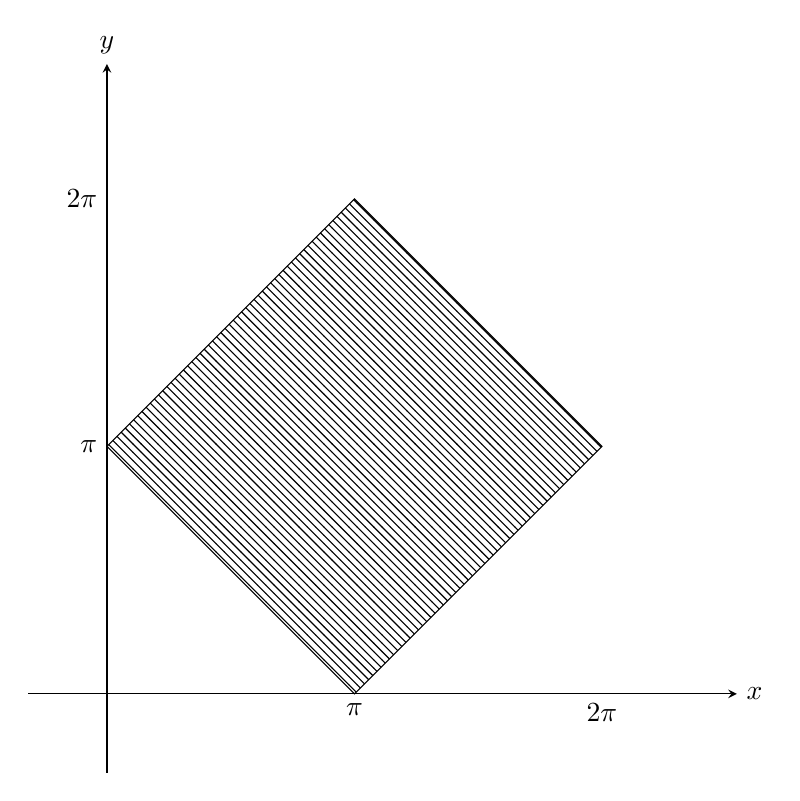
\begin{tikzpicture}
			\def\xMIN{-1};
			\def\xMAX{8};
			\def\yMIN{-1};
			\def\yMAX{8};

			\def\PI{22/7};

			\begin{scope}[-stealth]
				\draw (\xMIN,0) -- (\xMAX,0) node [right] {$x$};
				\draw (0,\yMIN) -- (0,\yMAX) node [above] {$y$};
			\end{scope}

			\begin{scope}
				\draw [fill, pattern = north west lines] (\PI,0) -- (2*\PI,\PI) -- (\PI,2*\PI) -- (0,\PI) -- cycle;
			\end{scope}

			\begin{scope}
				\node [below] at (\PI,0) {$\pi$};
				\node [below] at (2*\PI,0) {$2 \pi$};

				\node [left] at (0,\PI) {$\pi$};
				\node [left] at (0,2*\PI) {$2 \pi$};
			\end{scope}
		\end{tikzpicture}
	\end{figure}
\end{question}

\begin{solution}
	The edges of the domain are
	\begin{align*}
		x + y & = \pi   \\
		x + y & = 3 \pi \\
		x - y & = \pi   \\
		x - y & = -\pi
	\end{align*}
	Therefore, let
	\begin{align*}
		x - y & = u \\
		x + y & = v
	\end{align*}
	Therefore,
	\begin{align*}
		x & = \frac{u + v}{2} \\
		y & = \frac{v - u}{2}
	\end{align*}
	Therefore, the domain $R$ can be written as $S = \{-\pi \le u \le \pi, \pi \le v \le 3 \pi\}$.\\
	Therefore,
	\begin{align*}
		J &=
			\begin{pmatrix}
				x_u & x_v \\
				y_u & y_v \\
			\end{pmatrix}\\
		  &=
			\begin{pmatrix}
				\frac{1}{2}  & \frac{1}{2} \\
				-\frac{1}{2} & \frac{1}{2} \\
			\end{pmatrix}\\
		  &= \frac{1}{2}
	\end{align*}
	Therefore,
	\begin{align*}
		\iint\limits_{R} f(x,y) \dif x \dif y                              & = \iint\limits_{S} f\left( g(u,v), h(u,v) \right) |J| \dif u \dif v                                                   \\
		\therefore \iint\limits_{R} (x - y)^2 \sin^2 (x + y) \dif x \dif y & = \int\limits_{S} u^2 \sin^2 v \left| \frac{1}{2} \right| \dif u \dif v                                               \\
                                                                                   & = \frac{1}{2} \int\limits_{-\pi}^{\pi} \int\limits_{\pi}^{3 \pi} u^2 \sin^2 v \dif v \dif u                           \\
                                                                                   & = \frac{1}{2} \int\limits_{-\pi}^{\pi} u^2 \dif u \cdot \int\limits_{\pi}^{3 \pi} \sin^2 v \dif v                     \\
                                                                                   & = \frac{1}{2} \left. \frac{u^3}{3} \right|_{-\pi}^{\pi} \cdot \int\limits_{\pi}^{3 \pi} \frac{1 - \cos 2 v}{2} \dif v \\
                                                                                   & = \frac{1}{2} \frac{2 \pi^3}{3} \cdot \frac{1}{2} 2 \pi                                                               \\
                                                                                   & = \frac{\pi^4}{3}
	\end{align*}
\end{solution}

\subsection{Polar Coordinates}

Polar coordinates are a special case of change of variables.\\
The operator for the change of variables is
\begin{align*}
	T(r,\theta) & = (x,y)
\end{align*}
where
\begin{align*}
	x & = r \cos \theta \\
	y & = r \sin \theta
\end{align*}
Therefore,
\begin{align*}
	J &=
		\begin{vmatrix}
			x_r & x_{\theta} \\
			y_r & y_{\theta} \\
		\end{vmatrix}
	  &=
		\begin{vmatrix}
			\cos \theta & -r \sin \theta \\
			\sin \theta & r \cos \theta  \\
		\end{vmatrix}
	  &= r \cos^2 \theta + r \sin^2 \theta\\
	  &= r
\end{align*}

\begin{question}
	Calculate $\iint\limits_{R} x y \dif x \dif y$, $R = \left\{ (x,y) | 1 \le x^2 + y^2 \le 4 , 0 \le y \le x \right\}$.
\end{question}

\begin{solution}
	The domain $R$ is the region shown.
	\begin{figure}[H]
		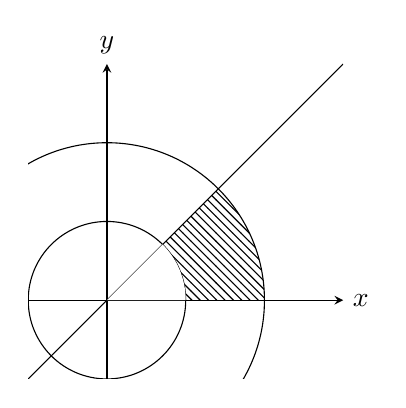
\begin{tikzpicture}
			\def\xMIN{-1};
			\def\xMAX{3};
			\def\yMIN{-1};
			\def\yMAX{3};

			\def\PI{22/7};

			\begin{scope}[-stealth]
				\draw (\xMIN,0) -- (\xMAX,0) node [right] {$x$};
				\draw (0,\yMIN) -- (0,\yMAX) node [above] {$y$};
			\end{scope}

			\begin{scope}
				\clip (\xMIN,\yMIN) rectangle (\xMAX,\yMAX);
				\draw (\xMIN,\yMIN) -- (\xMAX,\xMAX);
				\draw (0,0) circle (1);
				\draw (0,0) circle (2);
			\end{scope}

			\begin{scope}
				\clip (0,0) -- (\xMAX,\yMAX) -- (\xMAX,0) -- cycle;
				\fill [pattern = north west lines] (0,0) circle (2);
				\fill [white] (0,0) circle (1);
			\end{scope}
		\end{tikzpicture}
	\end{figure}
	Therefore, it can be written as $S = \left\{ (r,\theta) | 1 \le r \le 2 , 0 \le \theta \le \frac{\pi}{4} \right\}$.\\
	Therefore,
	\begin{align*}
		\iint\limits_{R} x y \dif x \dif y & = \int\limits_{0}^{\frac{\pi}{4}} \int\limits_{1}^{2} r \cos \theta r \sin \theta r \dif r \dif \theta     \\
                                                   & = \int\limits_{1}^{2} r^3 \dif r \cdot \int\limits_{0}^{\frac{\pi}{4}} \cos \theta \sin \theta \dif \theta \\
                                                   & = \frac{15}{4} \cdot \frac{1}{4}                                                                           \\
                                                   & = \frac{15}{16}
	\end{align*}
\end{solution}

\begin{theorem}
	Let $D$ be a domain, written as $D_{\mathrm{I}}$ in polar coordinates, i.e.,
	\begin{equation*}
		D_{\mathrm{I}} = \left\{ (r,\theta) | a \le r \le b , g_1(r) \le \theta \le g_2(r) \right\}
	\end{equation*}
	and let $f(x,y)$ be continuous on $D_{\mathrm{I}}$.\\
	Then,
	\begin{equation*}
		\iint\limits_{D_{\mathrm{I}}} f(x,y) \dif x \dif y = \int\limits_{a}^{b} \int\limits_{g_1(r)}^{g_2(r)} f(r \cos \theta, r \sin \theta) r \dif \theta \dif r
	\end{equation*}
\end{theorem}

\begin{theorem}
	Let $D$ be a domain, written as $D_{\mathrm{II}}$ in polar coordinates, i.e.,
	\begin{equation*}
		D_{\mathrm{I}} = \left\{ (r,\theta) | \alpha \le \theta \le \beta , h_1(\theta) \le r \le h_2(\theta) \right\}
	\end{equation*}
	and let $f(x,y)$ be continuous on $D_{\mathrm{II}}$.\\
	Then,
	\begin{equation*}
		\iint\limits_{D_{\mathrm{II}}} f(x,y) \dif x \dif y = \int\limits_{\alpha}^{\beta} \int\limits_{h_1(\theta)}^{h_2(\theta)} f(r \cos \theta, r \sin \theta) r \dif r\dif \theta
	\end{equation*}
\end{theorem}

\begin{question}
	Given $D = \left\{ x^2 + y^2 \le 2 x \right\}$, calculate $\iint\limits_{D} (x + y) \dif x \dif y$.
\end{question}

\begin{solution}
	\begin{align*}
		x^2 + y^2                  & = 2 x \\
		\therefore x^2 - 2 x + y^2 & = 0   \\
		\therefore (x - 1)^2       & = 1
	\end{align*}
	Therefore, the domain $D$ is as shown.
	\begin{figure}[H]
		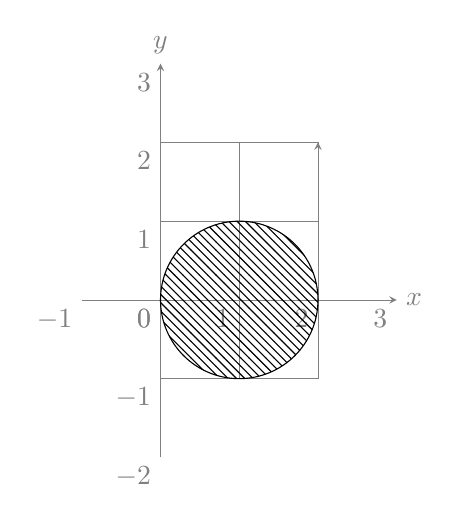
\begin{tikzpicture}
			\def\xMIN{-1};
			\def\xMAX{3};
			\def\yMIN{-2};
			\def\yMAX{3};

			\def\PI{22/7};

			\begin{scope}[-stealth, gray, very thin]
				\draw (\xMIN + 1,\yMIN + 1) grid (\xMAX - 1,\yMAX - 1);

				\foreach \x in {\xMIN,...,\xMAX}
				{
					\node [below left] at (\x,0) {$\x$};
				}

				\foreach \y in {\yMIN,...,\yMAX}
				{
					\node [below left] at (0,\y) {$\y$};
				}

				\draw (\xMIN,0) -- (\xMAX,0) node [right] {$x$};
				\draw (0,\yMIN) -- (0,\yMAX) node [above] {$y$};
			\end{scope}

			\begin{scope}
				\filldraw [pattern = north west lines] (1,0) circle (1);
			\end{scope}
		\end{tikzpicture}
	\end{figure}
	Therefore, $D$ can be written as $\left\{ 0 \le r \le 2 \cos \theta , -\frac{\pi}{2} \le \theta \le \frac{\pi}{2} \right\}$.\\
	Therefore,
	\begin{align*}
		\iint\limits_{D} (x + y) \dif x \dif y & = \int\limits_{-\frac{\pi}{2}}^{\frac{\pi}{2}} \int\limits_{0}^{2 \cos \theta} (r \cos \theta + r \sin \theta) r \dif r \dif \theta \\
                                                       & = \int\limits_{-\frac{\pi}{2}}^{\frac{\pi}{2}} (\cos \theta + \sin \theta) \left. \left( \frac{r^3}{3} \right) \right|_{z = 0}^{z = 2 \cos \theta} \dif \theta
	\end{align*}
	Solving,
	\begin{align*}
		\iint\limits_{D} (x + y) \dif x \dif y & = \pi
	\end{align*}
\end{solution}

\end{document}
